% ============================================================
%  Lizt: eBPF-Based Runtime Reachability Analysis for
%  Reducing False Positives in Software Composition Analysis
%
%  IEEEtran conference format
% ============================================================

\documentclass[conference]{IEEEtran}
\IEEEoverridecommandlockouts

% --- Standard packages ---
\usepackage[utf8]{inputenc}
\usepackage[T1]{fontenc}
\usepackage{cite}
\usepackage{amsmath,amssymb,amsfonts}
\usepackage{algorithmic}
\usepackage{graphicx}
\usepackage{textcomp}
\usepackage{xcolor}
% Better typography
\usepackage[protrusion=true,expansion=true]{microtype}
% Clickable refs/links (load hyperref late; before cleveref if used)
\usepackage{hyperref}
\usepackage{xurl}
% Code listings
\usepackage{listings}
% Better table rules (\toprule etc.)
\usepackage{booktabs}
\usepackage{fancyvrb}
% TikZ for diagrams
\usepackage{tikz}
\usetikzlibrary{positioning, arrows.meta, shapes.geometric,
                decorations.pathreplacing, fit, calc,
                backgrounds, patterns}
% Fine-grained list control
\usepackage{enumitem}
\usepackage{pgfplots}
\pgfplotsset{compat=1.18}
% Checkmark / cross symbols
\usepackage{pifont}
\newcommand{\cmark}{\ding{51}}
\newcommand{\xmark}{\ding{55}}

% Relaxed floating space for figures
\renewcommand{\topfraction}{0.9}
\renewcommand{\bottomfraction}{0.8}
\renewcommand{\textfraction}{0.1}
\renewcommand{\floatpagefraction}{0.8}

% --- Code listing style (Rust) ---
\definecolor{codebg}{RGB}{245,245,245}
\definecolor{codecomment}{RGB}{100,100,100}
\definecolor{codekeyword}{RGB}{0,0,180}
\definecolor{codestring}{RGB}{160,0,0}

\lstdefinelanguage{Rust}{
  keywords={fn, let, mut, pub, use, struct, enum, impl, trait, match, if, else, for, while, return, async, await, move, where, type, const, static, unsafe, mod, crate, self, super, true, false},
  keywordstyle=\color{codekeyword}\bfseries,
  comment=[l]{//},
  commentstyle=\color{codecomment}\itshape,
  stringstyle=\color{codestring},
  morestring=[b]",
  sensitive=true
}

\lstset{
  backgroundcolor=\color{codebg},
  basicstyle=\ttfamily\footnotesize,
  breaklines=true,
  frame=single,
  language=Rust,
  captionpos=b,
  numbers=left,
  numberstyle=\tiny\color{codecomment},
  numbersep=5pt
}

% ============================================================
\begin{document}
% ============================================================

% --- Title block ---
\title{Lizt: eBPF-Based Runtime Reachability Analysis\\
for Reducing False Positives in Software Composition Analysis}

\author{%
  \IEEEauthorblockN{Garrett Basil}
  \IEEEauthorblockA{%
    Georgia Institute of Technology \\
    Atlanta, Georgia, USA \\
    Email: gbasil3@gatech.edu%
  }%
}

\maketitle

% ============================================================
\begin{abstract}
  Software composition analysis (SCA) tools identify vulnerable dependencies by matching installed package versions against CVE
  databases, but this approach conflates the \emph{presence} of a
  vulnerable package with the \emph{reachability} of its vulnerable
  code at runtime. Prior work indicates 80--98\% of SCA findings may
  be operationally irrelevant as a result. We present \textit{Lizt},
  an open-source runtime reachability scanner that addresses this
  gap by layering eBPF uprobe monitoring on top of CPE/CVE matching:
  a CVE is promoted to a runtime-confirmed finding only when its
  associated symbols are both present in the target binary's dynamic
  symbol table and observed to execute during a workload. Lizt is
  implemented as a unified Cargo workspace in Rust using \texttt{aya}
  for eBPF, \texttt{axum} for a server-sent-events dashboard, and
  PostgreSQL as the sole coordination point between the scanner
  pipeline, the eBPF monitor, and the web frontend. We evaluate Lizt
  against a Grype baseline on three source-compiled fixtures
  (libexpat 2.2.9, OpenSSL 1.1.1f, zlib 1.2.11) covering five
  headline CVEs. Of 73 CPE-matched baseline findings, only 16 (21.9\%)
  carry runtime evidence of reachability under realistic workloads, a
  78\% reduction. A conditional-reachability experiment on
  CVE-2022-0778 further demonstrates that Lizt surfaces
  denial-of-service vulnerabilities identically on benign and
  malicious inputs, preserving the finding while leaving exploitability
  determination to the operator.
\end{abstract}


\begin{IEEEkeywords}
Software composition analysis, runtime reachability analysis,
eBPF uprobe monitoring, vulnerability detection,
dynamic analysis of vulnerable dependencies
\end{IEEEkeywords}

% ============================================================
\section{Introduction}
% ============================================================

Modern software systems are heavily dependent on third-party libraries, creating a large attack surface that is difficult to audit manually. Existing software composition analysis (SCA) tools such as Trivy~\cite{trivy} and Grype~\cite{grype} address this by matching installed packages with vulnerability databases (NVD~\cite{nvd}, OSV~\cite{osv}) using Common Platform Enumeration (CPE) identifiers. While effective in enumerating \textit{potential} exposure, this approach suffers from a fundamental limitation: a CPE match does not imply that the vulnerable code path exists in the compiled binary, let alone that it is ever executed at runtime. Previous work indicates that without analyzing reachability, 80--98\% of the SCA findings may be operationally irrelevant~\cite{konvu2026}.

This paper presents \textbf{Lizt}, an open-source runtime reachability scanner that addresses this gap. Lizt uses CPE/CVE matching only as a first-pass filter and layers eBPF-based uprobe monitoring as a confirmation stage. A CVE surfaces as an actionable finding only when the corresponding vulnerable symbol is observed to execute on the live system. This design follows a key insight: distro vendors frequently backport fixes without updating version strings, meaning that a package's reported version may match a CVE whose vulnerable code has already been patched out~\cite{redhat_backporting}. Symbol-level confirmation automatically detects these cases.

The primary contributions of this work are as follows.
\begin{itemize}[noitemsep]
  \item A five-stage SCA pipeline that composes inventory
        collection, NVD CVE ingestion with local version-range
        verification, multi-source symbol extraction, eBPF-based
        runtime monitoring, and a ranked findings dashboard, with
        symbol-level reachability exposed as a first-class triage
        signal through the \texttt{cpe\_match} /
        \texttt{symbol\_present} / \texttt{symbol\_called}
        three-level state.
  \item A symbol extraction subsystem that scrapes vulnerable
        function names from CVE descriptions, GitHub patch
        diffs and issues, and OSV records, with a multi-source
        corroboration heuristic that boosts confidence when
        independent sources agree, followed by binary-level
        validation against the target's dynamic symbol table
        before any probe is attached.
  \item A reproducible evaluation fixture system built on a
        \texttt{StaticSource} inventory provider and
        source-compiled vulnerable libraries installed under an
        isolated prefix, enabling head-to-head comparison against
        Grype on binaries that lack package-manager metadata.
  \item An empirical demonstration, on three source-compiled
        libraries and five headline CVEs, that 78\% of CPE-matched
        baseline findings lack runtime evidence of reachability
        under realistic workloads, and that the pipeline correctly
        surfaces conditional-reachability cases
        (CVE-2022-0778) on both benign and malicious inputs
        without collapsing the distinction into exploitability.
  \item An open-source implementation in Rust as a unified Cargo
        workspace producing a single \texttt{lizt} binary, using
        \texttt{aya}~\cite{aya}, \texttt{axum}, \texttt{sqlx}~\cite{sqlx},
        and PostgreSQL.
\end{itemize}


% ============================================================
\section{Background}
% ============================================================

\subsection{Existing Software Composition Analysis Dataflow}
For comparison, we first consider an existing tool in the SCA space: Anchore's Grype.

Grype first scans the target environment using a sister-tool called \textit{Syft}, which scans directories and files to build a software bill of materials (SBOM) contained within a specified parent directory or container image. It utilizes a pluggable set of catalogers to parse package metadata. For instance, Syft's \textit{dpkg-db-cataloger} parses \texttt{/var/lib/dpkg/status}, \textit{rpm-db-cataloger} parses \texttt{/var/lib/rpm/}, etc.

Grype's vulnerability database utilizes another sister-tool called \textit{Vunnel} to aggregate and transform data from multiple external vulnerability data sources into a form that is optimized for its own matching algorithm. At scan time, Grype downloads the most recent pre-built SQLite DB and performs matching locally.

To perform matching, Grype utilizes three distinct matching scenarios: distribution, GitHub security advisories, and NVD. If an item in the SBOM is an OS package installation, it utilizes that distribution security advisory feed to perform matching and determine potential vulnerabilities linked to that package. If the item is a language-specific installation (for example, one installed via \texttt{npm}), GitHub's security advisories are used. Finally, if the item is neither (e.g., it was installed from source, or via another distribution-independent manager like \texttt{homebrew}), CPE matching using the NVD is the fallback.

\subsection{CPE/CVE Matching}

Lizt's CPE/CVE matching layer is built on two NVD primitives: Common Platform Enumeration (CPE) identifiers and the NVD 2.0 REST API. A CPE is a colon-separated 13-field identifier~\cite{cpe_spec}; Lizt uses four of the fields---\texttt{part}, \texttt{vendor}, \texttt{product}, and \texttt{version}---and leaves the rest as wildcards. The NVD API exposes a CPE dictionary endpoint (used during inventory resolution to confirm a candidate string matches a known platform) and a CVE lookup endpoint that returns all vulnerabilities referencing a given \texttt{cpeName}.

Each CVE record's \texttt{configurations} block associates the vulnerability with impacted CPE ranges via \texttt{cpeMatch} entries. A match entry carries a CPE URI and up to four version boundaries: \texttt{versionStart\{Including,Excluding\}} and \texttt{versionEnd\{Including,Excluding\}}. For example, CVE-2022-37434 (zlib heap-based buffer overflow) uses a single entry with \texttt{versionEndExcluding} set to \texttt{1.2.12}, flagging all prior versions. Nodes can be composed with \texttt{AND}/\texttt{OR} to express cross-product applicability (e.g., a library vulnerable only on a specific OS); Lizt flattens these into independent match entries as a deliberate over-approximation, since the downstream eBPF stage is designed to filter spurious matches.

The NVD rate-limits unauthenticated clients to 5 requests per 30-second window and keyed clients to 50; Lizt implements a token-bucket scheduler that respects whichever window applies, with a bounded retry loop on \texttt{403} and \texttt{429} responses.

\subsubsection{Rate Limiting}

The NVD API imposes rate limitations on both endpoints. Unathenticated clients are limited to five requests per 30-second rolling window; obtaining a free API key increases the limit to fifty requests per 30-second window. A comprehensive inventory scan may identify numerous CPE candidates and then query the CVEs for each validated item.

\subsubsection{The Version-Range False Positive Problem}

CPE/CVE matching is fundamentally version-centric: if the installed version string lies within a CVE's specified vulnerable range, the package is marked as susceptible, irrespective of whether the underlying vulnerability persists in the compiled binary. This results in false positives in a minimum of two prevalent cases.

Initially, distribution vendors consistently \textit{backport} security patches to previous package versions without modifying the upstream version string~\cite{redhat_backporting}. Even if a Debian or Ubuntu system has the CVE-2022-37434 fix included in its zlib~1.2.11 package, a CPE-based scanner will check the version against the NVD range and report the vulnerability. The scanner cannot tell whether the vulnerable code path has been rectified, specifically the \texttt{inflateGetHeader} function.

Additionally, not all code paths identified as vulnerable by a CVE entry are present in every deployment. A library might provide numerous access points, but a specific application might use only a subsection of them. Designating the entire library as vulnerable conflates the \textit{presence} of the package with the \textit{reachability} of the vulnerable function, hence exaggerating the finding count with elements that present no operational risk.

The two failure modes---backport-induced version mismatch and unreachable code paths---prompt Lizt's methodology to consider CPE matching as an initial filter and postpone verification to a symbol-level runtime observation phase (\S\ref{sec:ebpf}).

\subsection{eBPF and Uprobes}
\label{sec:ebpf}

eBPF refers to a technology stack that allows user-provided programs to run in the kernel context without the use of kernel modules. In order to protect the kernel, a static analysis engine known as the \textit{verifier} processes the proposed program before insertion to protect against common memory and performance issues, such as unbounded loops or execution, and invalid memory accesses. There are many types of eBPF programs, but the two most relevant in the context of this work are \texttt{kprobe}, for kernel function entry, and \texttt{uprobe} for user-space function entry. eBPF programs run in a kernel context, but are unable to directly transfer data to user-space like a syscall might. Typed shared data structures, called \textit{maps} , are used as a communication mechanism between the two contexts, with the probes typically writing information related to the event (e.g., a function entry point) for the user-space program to interpret. These may be hash maps, arrays, per-CPU arrays, and/or ring buffers.

\texttt{Uprobes} have several properties that make them particularly helpful in the context of detecting function entry points during runtime. First, they use zero overhead when not fired; the first byte of the probed instruction is replaced with a break point instruction (e.g., \texttt{int3} on \texttt{x86\_64} ) \cite{kernel_kprobes}  \cite{corbet_uprobes_2012}. Second, they support symbol-level granularity and per-process-level attachment. This means that the probe attaches to a specific named symbol in a specific ELF binary, running with a specific PID, which allows control over observation scope; the observer can be sure that the symbol observation occurred within the specific context they want to look at. Finally, no application modification is required. Unlike IAST agents or RASP hooks, \texttt{uprobes} are attached externally by the kernel, leaving the target binary unaware of their existence, meaning that no re-compilation of target binaries is necessary.

\subsection{Related Work}

Several adjacent disciplines address the issue of runtime-aware vulnerability assessment, although none occupy the specific space targeted by Lizt.

\textbf{IAST and RASP.}
Interactive Application Security Testing (IAST) instruments a running application to monitor data flow and control flow during testing, integrating elements of static and dynamic analysis to detect vulnerabilities with low false-positive rates. Contrast Security~\cite{contrast_iast} was the first to utilize this method, deploying language-specific agents that add sensors to the application at runtime through aspect-oriented programming. Runtime Application Self-Protection (RASP) extends the same instrumentation approach from detection to active blocking: agents built into the application runtime catch requests that are determined to be potentially malicious and stop them before they reach vulnerable code paths~\cite{gartner_rasp}. Both IAST and RASP depend on connecting into a managed runtime environment, the JVM, .NET CLR, Node.js event loop, or Python interpreter, and therefore make the assumption that the target application executes within such a runtime. Native binaries compiled from C or C++ lack an equivalent instrumentation surface, rendering these approaches inapplicable to the system-level libraries (e.g., \texttt{zlib}, \texttt{libexpat}, OpenSSL) that constitute Lizt's primary targets.

\textbf{Reachability-based SCA.}
Eclipse Steady~\cite{steady}, developed by SAP Security Research, is the most comparable to Lizt in the academic space. Steady compares the method signatures in Java archives with known fixes to detect vulnerabilities. Afterwards, it combines static call-graph analysis with dynamic JUnit and integration test traces to determine if the vulnerable method was reachable. Ponta et al. found that 88.8\% of OWASP Dependency-Check findings for code-level vulnerabilities, which Steady's method covers, were false positives \cite{ponta2020}. However, Steady only works for Java or Python apps that use build systems like Maven or Gradle, and can't presently handle native ELF binaries or C/C++ libraries that are pre-existing on the system.

Endor Labs~\cite{endorlabs}, in its commercial offering, builds static call graphs directly from the source code, allowing them to assess function-level reachability, encompassing both direct and indirect dependencies. Their current support spans Java, JavaScript, Python, Go, Kotlin, .NET, and Rust. Snyk~\cite{snyk} offers a similar reachability analysis for Java, JavaScript, and Python, returning to a composite risk score for unsupported languages. Both tools operate at build time on source or package-manager artifacts, and neither performs runtime observation. Orca Security~\cite{orca} supplements agentless static scanning with an eBPF-based sensor that identifies which packages are loaded into memory in running containers; however, this operates at package granularity rather than symbol granularity, is proprietary and is aimed at containerized cloud workloads rather than general-purpose systems.

\textbf{Gap.}
To the best of our knowledge, no existing open-source tool combines CVE metadata with symbol-level eBPF uprobe monitoring to confirm runtime reachability of vulnerable code paths in native binaries. Lizt addresses this gap: it inherits CPE/CVE matching as a first-pass filter from traditional SCA, borrows the reachability confirmation concept from Steady and the commercial tools above, but replaces agent injection and call-graph construction with external, zero-modification uprobe attachment at the kernel level.

% Table~\ref{tab:comparison} summarizes the feature differences across these tools.

% \begin{table*}[t]
%   \centering
%   \caption{Feature comparison of Lizt with related vulnerability
%     analysis tools. \cmark\ = supported, \xmark\ = not supported,
%     $\sim$ = partial support.}
%   \label{tab:comparison}
%   \begin{tabular}{lcccccc}
%     \toprule
%     \textbf{Tool / Approach}
%       & \textbf{\shortstack{Native binary\\support}}
%       & \textbf{\shortstack{No agent\\injection}}
%       & \textbf{\shortstack{Runtime\\confirmation}}
%       & \textbf{\shortstack{Symbol-level\\granularity}}
%       & \textbf{\shortstack{Open\\source}}
%       & \textbf{\shortstack{Language\\agnostic}} \\
%     \midrule
%     Grype~\cite{grype}
%       & $\sim$ & \cmark & \xmark & \xmark & \cmark & \cmark \\
%     Trivy~\cite{trivy}
%       & \xmark & \cmark & \xmark & \xmark & \cmark & \cmark \\
%     Contrast IAST~\cite{contrast_iast}
%       & \xmark & \xmark & \cmark & $\sim$ & \xmark & \xmark \\
%     Eclipse Steady~\cite{steady}
%       & \xmark & \xmark & \cmark & \cmark & \cmark & \xmark \\
%     Endor Labs~\cite{endorlabs}
%       & \xmark & \cmark & \xmark & \cmark & \xmark & $\sim$ \\
%     Snyk~\cite{snyk}
%       & \xmark & \cmark & \xmark & $\sim$ & \xmark & $\sim$ \\
%     Orca Security~\cite{orca}
%       & $\sim$ & \cmark & $\sim$ & \xmark & \xmark & \cmark \\
%     \midrule
%     \textbf{Lizt}
%       & \cmark & \cmark & \cmark & \cmark & \cmark & \cmark \\
%     \bottomrule
%   \end{tabular}
% \end{table*}

% ============================================================
\section{System Design}
% ============================================================
\label{sec:sysdesign}

Figure~\ref{fig:pipeline-expanded} shows Lizt's five-stage pipeline. Each stage is implemented as an independent crate within a Cargo workspace, with the \texttt{pipeline} crate acting as the sole public API surface consumed by the CLI and web frontends.

\begin{figure}[t]
  \centering
  \resizebox{\columnwidth}{!}{
  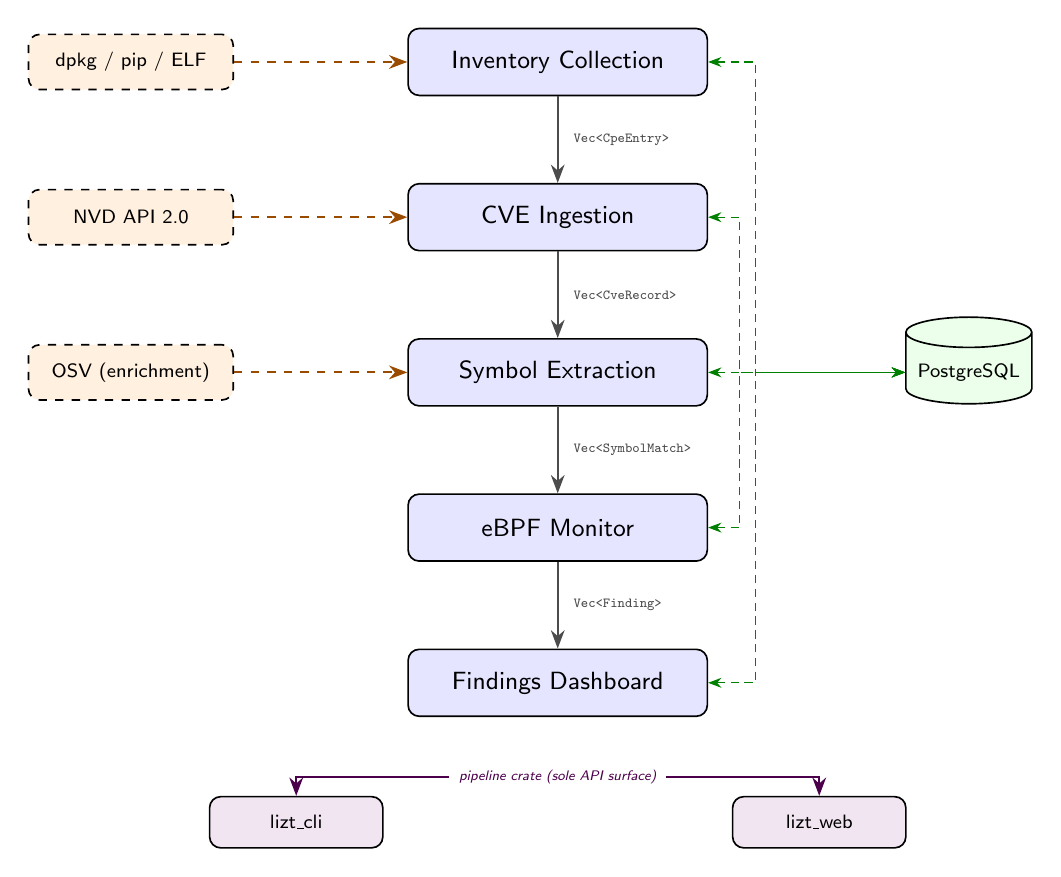
\begin{tikzpicture}[
      stage/.style={
          draw, rectangle, rounded corners=4pt,
          fill=blue!10, minimum width=3.8cm,
          minimum height=0.85cm, align=center,
          font=\small\sffamily, line width=0.6pt
        },
      ext/.style={
          draw, rectangle, rounded corners=4pt,
          fill=orange!12, minimum width=2.6cm,
          minimum height=0.7cm, align=center,
          font=\scriptsize\sffamily, line width=0.6pt,
          dashed
        },
      db/.style={
          draw, cylinder, shape border rotate=90,
          aspect=0.25, minimum height=1.1cm, minimum width=1.6cm,
          fill=green!8, font=\scriptsize\sffamily,
          line width=0.6pt
        },
      consumer/.style={
          draw, rectangle, rounded corners=4pt,
          fill=violet!10, minimum width=2.2cm,
          minimum height=0.65cm, align=center,
          font=\scriptsize\sffamily, line width=0.6pt
        },
      arrow/.style={->, thick, >=Stealth},
      dataarrow/.style={->, thick, >=Stealth, font=\tiny\ttfamily,
          color=black!70},
      dbarrow/.style={<->, densely dashed, >=Stealth,
          color=green!50!black, thin}
    ]

    % ── Pipeline stages (vertical) ──
    \node[stage] (inv)  {Inventory Collection};
    \node[stage, below=1.1cm of inv]  (cve)  {CVE Ingestion};
    \node[stage, below=1.1cm of cve]  (sym)  {Symbol Extraction};
    \node[stage, below=1.1cm of sym]  (ebpf) {eBPF Monitor};
    \node[stage, below=1.1cm of ebpf] (dash) {Findings Dashboard};

    % ── Arrows between stages with data annotations ──
    \draw[dataarrow] (inv)  -- node[right, xshift=2pt] {Vec<CpeEntry>} (cve);
    \draw[dataarrow] (cve)  -- node[right, xshift=2pt] {Vec<CveRecord>} (sym);
    \draw[dataarrow] (sym)  -- node[right, xshift=2pt] {Vec<SymbolMatch>} (ebpf);
    \draw[dataarrow] (ebpf) -- node[right, xshift=2pt] {Vec<Finding>} (dash);

    % ── External sources (left side) ──
    \node[ext, left=2.2cm of inv] (dpkg) {dpkg / pip / ELF};
    \node[ext, left=2.2cm of cve] (nvd)  {NVD API 2.0};
    \node[ext, left=2.2cm of sym] (osv)  {OSV (enrichment)};

    \draw[arrow, dashed, color=orange!60!black]
    (dpkg) -- (inv);
    \draw[arrow, dashed, color=orange!60!black]
    (nvd) -- (cve);
    \draw[arrow, dashed, color=orange!60!black]
    (osv) -- (sym);

    % ── PostgreSQL (right side) ──
    \node[db, right=2.5cm of sym] (pg) {PostgreSQL};

    \draw[dbarrow] (inv.east)  -- ++(0.6,0) |- (pg);
    \draw[dbarrow] (cve.east)  -- ++(0.4,0) |- (pg);
    \draw[dbarrow] (sym.east)  -- (pg);
    \draw[dbarrow] (ebpf.east) -- ++(0.4,0) |- (pg);
    \draw[dbarrow] (dash.east) -- ++(0.6,0) |- (pg);

    % ── Consumer frontends (below) ──
    \node[consumer, below left=1.0cm and 0.3cm of dash]  (cli) {lizt\_cli};
    \node[consumer, below right=1.0cm and 0.3cm of dash] (web) {lizt\_web};

    % ── Pipeline crate bracket ──
    \node[draw=none, below=0.55cm of dash, font=\tiny\sffamily\itshape,
      color=violet!60!black] (pipelab) {pipeline crate (sole API surface)};
    \draw[arrow, color=violet!60!black]
    (pipelab.west) -| (cli.north);
    \draw[arrow, color=violet!60!black]
    (pipelab.east) -| (web.north);

  \end{tikzpicture}
  }
  \caption{Lizt's five-stage pipeline with data flow annotations.
    Dashed lines indicate external data sources; double-headed
    arrows show database read/write paths. Both CLI and web
    frontends consume the \texttt{pipeline} crate as a single
    API surface.}
  \label{fig:pipeline-expanded}
\end{figure}

\subsection{Inventory Collection}
Lizt models inventory sources using a \texttt{Source} trait with a single \texttt{collect()} method returning a \texttt{Vec} of a common \texttt{CpeEntry} class type. Four initial sources are provided: \texttt{UbuntuSource} parses \texttt{/etc/os-release} to produce a CPE entry for the host OS (\emph{High}), \texttt{LinuxKernelSource} extracts a cleaned kernel version from \texttt{uname -r} (\emph{High}), \texttt{DpkgSource} parses \texttt{dpkg-query} output for Debian/Ubuntu system packages while skipping \texttt{python-}-prefixed entries to avoid duplication with pip (\emph{Medium}), and \texttt{PipSource} parses \texttt{pip list --format=json} for Python packages installed outside \texttt{apt} (\emph{Low}, since CPE \texttt{vendor} fields cannot be reliably inferred). The \texttt{InventoryItemConfidence} tier feeds downstream prioritization.

Prior to matching, the \texttt{Inventory} collector applies two normalization processes. First, a version-cleanup pipeline removes things like Debian epoch prefixes, distribution suffixes (e.g., \texttt{dfsg}, \texttt{ubuntu}, etc.), build IDs and trailing extraversion numbers to provide the matching algorithm with a best-guess of the upstream version string expected by the NVD. Second, an alternative-CPE generator produces additional candidate entries with common naming variations (such as removing \texttt{lib} prefixes), since NVD product names are not always consistent with distribution package names. A \texttt{HashSet} is keyed on the formatted CPE strings to perform removal of duplicates, and only those that resolve against the NVD inventory of CPE strings are maintained into the CVE ingestion stage to prevent wasteful queries.

A fifth source, \texttt{StaticSource} handles the evaluation fixture system inventory (\S\ref{sec:fixtures}), and accepts hard coded \texttt{CpeEntry} items to inject known-vulnerable software versions into the pipeline without requiring the corresponding packages to be installed outside of a sandboxed area of the host.

\subsection{CVE Ingestion}
Once inventory collection produces a set of validated CPE entries, Lizt queries the NVD CVE API (\texttt{/cves/2.0}) using each CPE string as a \texttt{cpeName} parameter. The NVD endpoint returns any CVE records containing a \texttt{configurations} block that references the provided CPE string, including records with version ranges that do not actually contain the installed version. Lizt follows \texttt{startIndex}-based pagination until all results are exhausted. A token-bucket rate-limiting scheme is implemented to respect NVD's 5-per-30-second window without an API key or 50-per-30-second window with one. To account for network instability or other factors outside Lizt's control, a retry loop is implemented within the REST request logic with a bounded number of attempts. For \texttt{403} or \texttt{429} responses indicating that the rate-limiting rules are in effect, sleeps are performed before retrying.

As a result of the unreliable nature of CPE version matching mentioned above, Lizt applies a local version-range verifier using its own comparator. Version strings are first tokenized by splitting on \texttt{the.} and \texttt{-} delimiters, and the components are segmented into numeric and alphabetic tokens. Numeric tokens are compared as integers and alphabetic tokens are lexicographically compared. Numeric tokens are considered "higher" than alphabetic tokens in the same position. This scheme allows for more diverse versioning conventions without requiring strict semantic versioning adherence. (e.g., OpenSSL's letter suffixed versions \texttt{1.1.1f} $<$ \texttt{1.1.1g} are sorted correctly).
The comparator accounts for all four NVD boundary fields: \texttt{versionStartIncluding}, \texttt{versionStartExcluding}, \texttt{versionEndIncluding}, and \texttt{versionEndExcluding} when determining whether or not the installed version falls within the range specified by the NVD record. If the comparator fails, the result is discarded. This serves to both eliminate false matches and reduce downstream noise.

Once a CVE is matched, its ID is used as an input to the Open Source Vulnerabilities (OSV) distributed database endpoint, providing additional and potentially enriched information about the vulnerability. Selected metadata (the description text, publication date, CVSS scores, references, etc.) from the matched CVEs are stored in a  PostgreSQL database.

In the process of transforming NVD answers into internal \texttt{Cve} structures, Lizt consolidates all configuration nodes into a singular list of \texttt{CveCpe} match entries, eliminating the node-level \texttt{AND} and \texttt{OR} operators. This constitutes a calculated over-approximation: AND-gated setups (e.g., a library vulnerability pertinent solely to a certain operating system) are regarded as if each match item separately signifies vulnerability. The architecture permits more false positives at this step, which the subsequent eBPF confirmation stage is explicitly intended to filter, rather than jeopardize false negatives from inaccurately assessing sophisticated multi-node applicability logic. Accurate AND-node evaluation necessitates cross-referencing the complete system inventory with each node in a configuration, which is designated as future work.

\subsection{Symbol Extraction}

The symbol extraction stage identifies the potential function names associated with each CVE later used by the eBPF monitor as the instrumentation point. Lizt scrapes four logical sources, implemented as three \texttt{Scraper} trait objects run concurrently per CVE via \texttt{futures::future::join\_all}. Table~\ref{tab:symbol-sources} summarizes the sources and their confidence assignments.

\begin{table*}[h]
  \centering
  \label{tab:symbol-sources}
  \begin{tabular}{llc}
    \toprule
    \textbf{Source}        & \textbf{Method}                        & \textbf{Confidence} \\
    \midrule
    CVE description        & Regex pattern matching                 & Medium / Low        \\
    GitHub commit diff     & Function definition \& call-site parse & High / Low          \\
    GitHub issue / PR      & Title + body text (description regex)  & Medium / Low        \\
    OSV database           & Patch diffs + details text             & High / Low          \\
    \bottomrule
  \end{tabular}
  \caption{Symbol extraction sources and confidence tiers. The GitHub scraper covers two source types internally.}
\end{table*}

\paragraph{Description scraper}
The description scraper uses six regex-based rules based on common patterns to search CVE description text for function name candidates. Parenthesized identifiers (e.g., \texttt{inflate()}) receive \textit{Medium} confidence. Backtick-quoted identifiers, keyword-adjacent names ("vulnerable function \texttt{foo}"), and reverse-order variants ("\texttt{foo} vulnerable function") receive \textit{Low} to reduce the number of false positive matches (as \textit{Low} confidence matches are filtered out before instrumentation). An "in $\langle$function$\rangle$" pattern captures prose references common in kernel advisories and matches kernel-prefixed symbols (\texttt{\_\_*}, \texttt{tcp\_*}, \texttt{ext4\_*}, etc.). Finally, symbols matching a curated list of well-known API prefixes (e.g. SSL \_, \texttt{BN \_}, \texttt{inflate}, \texttt{XML} \texttt{\_}) are boosted from \textit{Low} to \textit{Medium} to prevent premature filtering.

\paragraph{GitHub scraper}
When NVD reference data includes URLs tagged as \texttt{Patch}, the GitHub scraper prioritizes those links and skips references tagged only as \texttt{Press/Media~Coverage} or \texttt{Exploit}, reducing wasted API rate-limit budget. This is particularly important for GitHub requests, where the reset window is a full hour (albeit with a much higher number of allowed requests per window at 5000)\cite{github_rate_limits}. For commit diffs, the scraper uses language-specific function definition regexes for C, Python, Java, Rust, and Go. It gives \textit{High} confidence to matches on definition sites. Changed lines (unified diff additions and deletions) are additionally scanned for generic call-site patterns (\texttt{name(...)}), assigned \textit{Low} confidence since these matches are inherently noisier. Files with paths that match common test or example directory conventions (\texttt{tests/}, files ending with \texttt{\_test.c}, \texttt{examples/}, etc.) are excluded. The scraper combines the title and body text for issues and pull requests and uses the same regex rules as the description scraper.

\paragraph{OSV scraper}
The OSV scraper queries the OSV database for information using existing CVE IDs in the pipeline. The OSV response includes organized \texttt{fix} events that provide patch commit URLs. The same diff parser utilized by the GitHub scraper is employed to fetch and process these URLs. When the OSV \texttt{details} field is present, the description scraper uses regex rules for processing.

\paragraph{Deduplication and confidence boosting}
Because the same symbol may appear across multiple sources for a single CVE, the extractor deduplicates by grouping on the composite key \texttt{(name, cve\_id)}. Within each group, the highest-confidence match is retained. The extractor also tracks distinct source type prefixes (e.g. description, \texttt{commit} \_diff, \texttt{github} \texttt{\_issue}) per group; if two or more distinct source types independently identified the same symbol, the confidence of the retained symbol is increased by one level (Low~$\to$ ~ Medium, Medium~$\to$ ~ High). This multi-source corroboration heuristic reflects the intuition that a symbol mentioned in both a CVE description and a patch commit is more likely to be the actual vulnerable entry point.

\paragraph{Filtering}
After deduplication, a validation pass retains only symbols satisfying two criteria: the name must pass a plausibility filter (\texttt{is\_likely\_function\_name}), and the confidence must be at least \textit{Medium}. The plausibility filter rejects English stop words, C type names (\texttt{size\_t}, \texttt{uint32\_t}), ALL\_CAPS macro-style identifiers exceeding six characters (unless they are prefixed by kernel-style double-underscores), file paths (containing forward slashes), version strings, digit-prefixed names, and names shorter than three characters. An early design included a \texttt{SymbolType} enum to distinguish functions from macros and variables; this was removed because kprobes and uprobes attach to executable instruction addresses resolved from symbol names~\cite{kernel_kprobes, kernel_uprobes}; macros have no presence in the compiled binary, and variables are data addresses, not instruction entry points, and all four scrapers already produce only function-shaped patterns, making the distinction purely taxonomic.

\paragraph{Language inference}
Scrapers assign a source language when the syntactic context is unambiguous (e.g., \texttt{def foo()} implies Python, \texttt{fn foo()} implies Rust). For symbols left as \textit{Unknown}, the extractor performs a second pass using CPE and description hints: a CPE product of \texttt{linux\_kernel} implies \textit{Kernel}, and description keywords such as \texttt{openssl} or \texttt{glibc} imply \textit{C}. Although this heuristic does not affect the probe attachment directly, it provides useful metadata for triage in the findings dashboard.

\paragraph{Symbol validation}
Before symbols can be instrumented, they must be confirmed present on the target system. The pipeline builds a \texttt{SymbolIndex} by scanning two sources: \texttt{/proc/kallsyms} for kernel symbols (kprobe candidates) and the dynamic symbol tables of installed library files for userspace symbols (uprobe candidates). The path of candidate library files are resolved via \texttt{dpkg}, \texttt{pip}, or static path conventions, depending on the inventory source that originally reported the package. Exported symbols are enumerated using \texttt{nm~--defined-only}. Each extracted symbol is used to query its row in the database; matches are annotated with a \texttt{binary\_path}, a \texttt{probe\_type} (kprobe or uprobe), and a \texttt{validated} flag set to \texttt{TRUE}. Only validated symbols are forwarded to the eBPF monitor; invalidated symbols are retained in the database for audit-ability but excluded from instrumentation.

\subsection{eBPF Monitoring}
The monitoring stage consumes the validated symbol set produced by the extraction pipeline and attaches eBPF probes to observe whether those symbols execute at runtime. The functionality is split between two crates: the \texttt{ebpf\_programs} crate compiled to the \texttt{bpfel-unknown-none} target using the Aya eBPF framework~\cite{aya}, and a userspace \texttt{monitor} library that loads the compiled bytecode, attaches probes, and collects events. The kernel-side bytecode is embedded directly into the host binary at build time using \texttt{aya::include\_bytes\_aligned!} rather than deploying a separate BPF object file.

A single BPF program cannot determine which symbol triggered it when attached to multiple entry points. Lizt therefore loads a \emph{separate} BPF program instance for each validated symbol. Before each instance is loaded into the kernel, the loader stamps the symbol's database primary key into a read-only global variable (\texttt{CVE\_SYMBOL\_ID}) via \texttt{EbpfLoader::set\_global}. The program is then attached as either a \texttt{kprobe} or \texttt{uprobe} depending on the \texttt{probe\_type} annotation set during symbol validation: kernel symbols discovered in \texttt{/proc/kallsyms} are attached via \texttt{KProbe::attach}, while userspace symbols carry a resolved \texttt{binary\_path} and are attached via \texttt{UProbe::attach} to the corresponding shared object.

Every BPF program has its own 256 KiB ring buffer map. When a probed symbol is executed during runtime, the kernel-side handler makes room in the ring buffer and writes a fixed-layout \texttt{Event} containing the calling process's PID, thread group ID, 16-byte process name (\texttt{comm}) and the stamped \texttt{cve\_symbol\_id}. The monitor creates one asynchronous Tokio task for each probe on the userspace side. Each task uses a \texttt{tokio::io::unix::AsyncFd} to wrap the ring buffer's file descriptor so that it can get kernel readiness notifications without busy-polling. When the task wakes up, it drains any events that are available and upserts each observation into a \texttt{symbol\_observations} table in PostgreSQL.

The monitor listens to the pipeline's \texttt{tokio::sync::broadcast} channel for \texttt{ScanEvent::Complete} signals. When a scan finishes, potentially adding new validated symbols, the monitor tears down all existing probes and reloads the full set from the database, ensuring that newly discovered symbols are instrumented without requiring a process restart. A capability check at startup verifies that the process holds \texttt{CAP\_BPF}, \texttt{CAP\_PERFMON}, and \texttt{CAP\_SYS\_RESOURCE} by inspecting \texttt{/proc/self/status}; if any are missing, the monitor logs a diagnostic and exits gracefully rather than failing at the first \texttt{attach} call.

Probe attachment can be verified externally via \texttt{bpftool prog list}, which enumerates all loaded BPF programs and their attachment points, and \texttt{/sys/kernel/debug/tracing/uprobe\_events}, which lists active uprobe registrations by binary path and symbol offset.

Figure~\ref{fig:uprobe-lifecycle} traces the event path from uprobe firing to dashboard delivery.

\begin{figure*}[t]
  \centering
  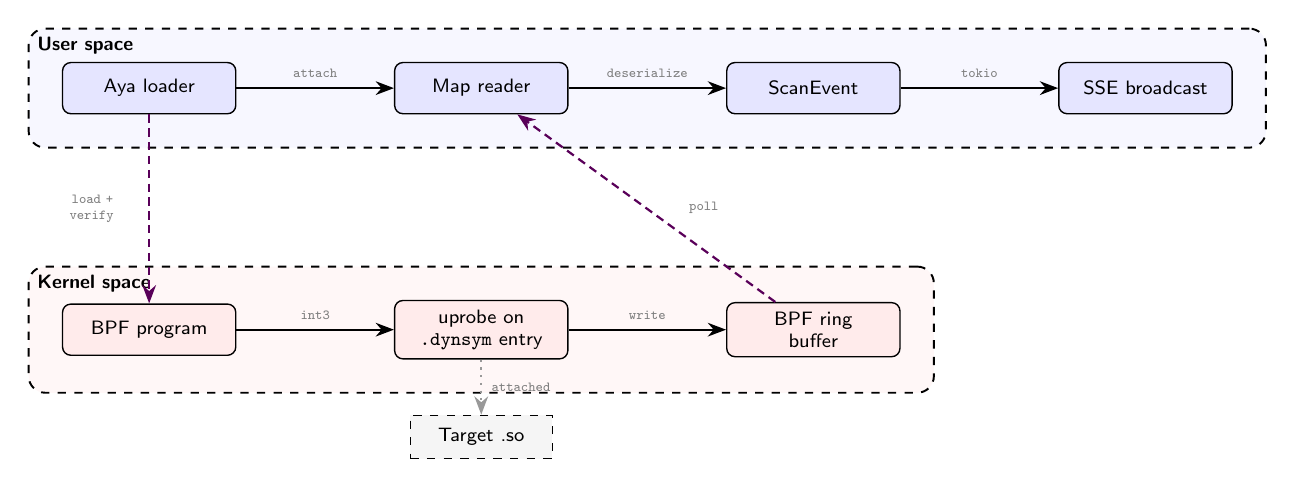
\begin{tikzpicture}[
    box/.style={
      draw, rectangle, rounded corners=3pt,
      minimum height=0.65cm, align=center,
      font=\scriptsize\sffamily, line width=0.5pt,
      minimum width=2.2cm
    },
    kbox/.style={box, fill=red!8},
    ubox/.style={box, fill=blue!10},
    zone/.style={
      draw, dashed, rounded corners=6pt,
      line width=0.7pt, inner sep=12pt
    },
    arrow/.style={->, thick, >=Stealth},
    annot/.style={font=\tiny\ttfamily, color=black!50}
  ]

    % ── User space zone ──
    \node[ubox] (aya) {Aya loader};
    \node[ubox, right=2.0cm of aya] (mapread) {Map reader};
    \node[ubox, right=2.0cm of mapread] (event) {ScanEvent};
    \node[ubox, right=2.0cm of event] (sse) {SSE broadcast};

    \draw[arrow] (aya) -- node[above, annot] {attach} (mapread);
    \draw[arrow] (mapread) -- node[above, annot] {deserialize} (event);
    \draw[arrow] (event) -- node[above, annot] {tokio} (sse);

    \begin{scope}[on background layer]
      \node[zone, fill=blue!3,
            fit=(aya)(mapread)(event)(sse),
            label={[font=\scriptsize\sffamily\bfseries,
                    anchor=north west]north west:User space}] {};
    \end{scope}

    % ── Kernel space zone ──
    \node[kbox, below=2.4cm of aya] (bpfprog) {BPF program};
    \node[kbox, right=2.0cm of bpfprog] (uprobe)
      {uprobe on \\ \texttt{.dynsym} entry};
    \node[kbox, right=2.0cm of uprobe] (map) {BPF ring \\ buffer};

    \draw[arrow] (bpfprog) -- node[above, annot] {int3} (uprobe);
    \draw[arrow] (uprobe) -- node[above, annot] {write} (map);

    \begin{scope}[on background layer]
      \node[zone, fill=red!3,
            fit=(bpfprog)(uprobe)(map),
            label={[font=\scriptsize\sffamily\bfseries,
                    anchor=north west]north west:Kernel space}] {};
    \end{scope}

    % ── Cross-boundary arrows ──
    \draw[arrow, densely dashed, color=violet!70!black]
      (aya) -- node[left, annot, text width=1.2cm, align=center]
      {load +\\verify} (bpfprog);
    \draw[arrow, densely dashed, color=violet!70!black]
      (map) -- node[right, annot, text width=1.2cm, align=center]
      {poll} (mapread);

    % ── Target binary ──
    \node[draw, rectangle, dashed, fill=gray!8,
          minimum width=1.8cm, minimum height=0.55cm,
          font=\scriptsize\sffamily,
          below=0.7cm of uprobe] (target) {Target .so};
    \draw[arrow, dotted, color=black!40] (uprobe) --
      node[right, annot] {attached} (target);

  \end{tikzpicture}
  \caption{Uprobe lifecycle. The Aya loader compiles, verifies,
    and attaches the BPF program to a symbol in the target
    binary's \texttt{.dynsym}. When the symbol executes, the
    kernel fires the uprobe and writes an event to a ring buffer.
    The user-space map reader deserializes the event into a
    \texttt{ScanEvent} and broadcasts it to the dashboard via
    SSE over a \texttt{tokio::sync::broadcast} channel.}
  \label{fig:uprobe-lifecycle}
\end{figure*}

\subsection{Findings Dashboard}

The findings dashboard is served by an Axum-based HTTP server that exposes a JSON REST API and a single-page HTML frontend. Scan progress is delivered to the browser in real time via server-sent events (SSE): the \texttt{pipeline} crate emits \texttt{ScanEvent} variants (\texttt{Started}, \texttt{Stage}, \texttt{Complete}, \texttt{Failed}) over a \texttt{tokio::sync::broadcast} channel, and the web layer wraps a \texttt{BroadcastStream} subscriber into an Axum \texttt{Sse} response. The frontend consumes these events to render a live stage-tracker that advances through the pipeline stages as the scan progresses and surfaces errors immediately on failure.

The Findings are ranked by a \texttt{computed \_rank \_score} SQL function that combines static severity indicators: CVSS base score, membership in the CISA Known Exploited Vulnerabilities (KEV) catalog and EPSS probability, with the runtime signal from the eBPF monitor. When at least one symbol associated with a CVE has been observed at runtime, the \texttt{symbol\_called} flag on the finding is set and the rank score is boosted, surfacing runtime-confirmed vulnerabilities above those that remain unobserved. This ranking is the mechanism by which the eBPF monitor's observations translate into actionable triage priority.

For deployment on shared infrastructure, an nginx reverse proxy sits in front of the Axum server to provide TLS termination via Let's Encrypt certificates and HTTP basic authentication. Both the web server and the eBPF monitor run within a single \texttt{lizt} binary managed as a systemd service, with ambient capabilities (\texttt{CAP\_BPF}, \texttt{CAP\_PERFMON}, \texttt{CAP\_SYS\_RESOURCE}) granted via the unit file so that the process does not need to run as root. PostgreSQL serves as the sole coordination point between the scanner pipeline, the eBPF monitor, and the dashboard: scan results, symbol observations, and ranked findings flow through the shared database.



% ============================================================
\section{Implementation}
% ============================================================

\subsection{Workspace Structure}
\label{sec:workspace}

Lizt is implemented as a single unified Cargo workspace producing one \texttt{lizt} binary. An earlier design split the project into two workspaces---a stable-Rust scanner and a nightly-Rust eBPF monitor---to isolate the \texttt{bpf-linker} toolchain requirement. This boundary was ultimately consolidated: the Aya framework compiles its eBPF programs from a dedicated \texttt{monitor-ebpf} sub-crate at build time and embeds the resulting bytecode into the host binary via \texttt{aya::include\_bytes\_aligned!}, so the nightly toolchain is required only for the eBPF sub-crate and does not need to propagate across a workspace boundary. Collapsing the two workspaces eliminated a class of cross-workspace dependency duplication (shared types in \texttt{core/common}, shared queries in \texttt{core/db}) and allowed the web server and the eBPF monitor to run as a single process under a single systemd service, using PostgreSQL as their sole coordination point (\S\ref{sec:database}).

The workspace is partitioned into four logical layers. The \textbf{core} layer (\texttt{core/common}, \texttt{core/db}) provides the shared domain types and the sqlx-backed persistence layer consumed by every other crate. The \textbf{io} layer (\texttt{io/inventory}, \texttt{io/nvd}, \texttt{io/symbols}) isolates all external I/O: filesystem and package-manager probing, NVD and OSV HTTP clients, and the symbol scrapers. The \textbf{pipeline} crate orchestrates the five stages described in \S\ref{sec:sysdesign} and serves as the only public API surface for consumers. The \textbf{consumer} layer contains the three entry points: \texttt{scanner/cli} (a Clap-based CLI with \texttt{inquire} for interactive prompts and CSV export), \texttt{scanner/web} (the Axum HTTP server and SSE dashboard) and \texttt{monitor} (the Aya-based eBPF loader, which runs as a background task spawned by \texttt{scanner/web}). An additional \texttt{xtask} crate~\cite{xtask} provides task automation (\texttt{cargo xtask build-ebpf}, \texttt{cargo xtask test}) without introducing a shell-script dependency.

The crate dependency layering is strict: consumer crates depend on \texttt{pipeline} but never directly on \texttt{io} crates, and the \texttt{io} crates depend only on \texttt{core/common}, not on \texttt{core/db}. This keeps I/O adapters free of persistence concerns and makes the \texttt{pipeline} crate the single aggregation point between data acquisition and storage.

Shared external dependencies (\texttt{tokio}, \texttt{serde}, \texttt{sqlx}, \texttt{log}) are declared once in the root \texttt{Cargo.toml} under \texttt{[workspace.dependencies]} and inherited by member crates via \texttt{\{ workspace = true \}}. This prevents version skew across crates and keeps the per-crate manifests short. Internal crates use the same inheritance pattern for their own version and authorship fields.

The eBPF programs themselves live in a \texttt{monitor-ebpf} sub-crate, built with the \texttt{bpfel-unknown-none} target using \texttt{aya-build} driven from \texttt{monitor}'s \texttt{build.rs}. To keep rust-analyzer responsive in VS~Code, a \texttt{monitor/.vscode/settings.json} file pins the target for the eBPF sub-crate only, allowing the rest of the workspace to retain the default host target.

% ============================================================
\subsection{Database Layer}
\label{sec:database}

PostgreSQL serves as both the persistence backend and the sole coordination point between the scanner pipeline, the eBPF monitor, and the findings dashboard. All database access is mediated by the \texttt{core/db} crate using \texttt{sqlx}~\cite{sqlx} with compile-time query verification: queries are checked against a live PostgreSQL instance at build time, and any schema drift surfaces as a compilation error rather than a runtime exception.

\subsubsection{Schema Overview}

The schema comprises seven tables and one materialized view. Three roles are played by the tables: \emph{inventory state} (\texttt{cpes}), \emph{vulnerability knowledge} (\texttt{cves}, \texttt{kev}, \texttt{cve\_symbols}), and \emph{scan-scoped results} (\texttt{scans}, \texttt{findings}, \texttt{symbol\_observations}).

The \texttt{cpes} table holds inventory items keyed by \texttt{(name, product)}. The \texttt{cpe} column is nullable because NVD CPE resolution may fail for packages absent from the dictionary; such rows are retained for audit but skipped by the CVE ingestion stage. The \texttt{cpe\_confidence} column records the \texttt{InventoryItemConfidence} tier assigned by the source (\S\ref{sec:sysdesign}).

The \texttt{cves} table holds the union of all CVEs ever matched against any inventory item, with CVSS and EPSS~\cite{epss} scoring, publication metadata, and the raw \texttt{references} block as \texttt{JSONB} for downstream mining by the symbol scraper. The \texttt{kev} table~\cite{cisa_kev} is a simple membership table whose presence acts as a boolean flag in the ranking function. The \texttt{cve\_symbols} table holds scraped symbols with their confidence tier, source lang, and---once symbol validation has run---the resolved \texttt{binary\_path} and \texttt{probe\_type} (\S\ref{sec:sysdesign}). A partial index over \texttt{validated} rows keeps the hot path for the eBPF loader's startup query fast.

The \texttt{scans} table anchors every pipeline run. Its \texttt{fixture\_name} column is the mechanism by which evaluation runs are distinguished from production scans: \texttt{NULL} identifies a real system scan, while a non-\texttt{NULL} value names the fixture being exercised. All downstream tables (\texttt{findings}, \texttt{symbol\_observations} via \texttt{cve\_symbols}) inherit the scan's identity through foreign-key chains, so fixture data and production data can coexist in the same database without a separate schema.

The \texttt{findings} table is the join point between inventory and vulnerability knowledge, with a uniqueness constraint on \texttt{(scan\_id, cpe\_id, cve\_id)} preventing duplicates within a single scan. The \texttt{cpe\_match} and \texttt{symbol\_present} columns encode the static portion of the reachability state: version-range match and symbol presence in the binary's symbol tables. The runtime-called state is derived on demand from \texttt{symbol\_observations} via an \texttt{EXISTS} subquery materialized into the API response, keeping the hot uprobe-fire path free of \texttt{findings}-table writes and allowing the ranking function to be evaluated against the freshest observation data.

\subsubsection{Observation Upserts and Materialized Activity}

The \texttt{symbol\_observations} table has a uniqueness constraint on \texttt{(cve\_symbol\_id, pid)} and a \texttt{call\_count} column that is incremented on conflict, allowing the eBPF monitor to upsert every observation without materializing a row per uprobe firing. This matters under load: a uprobe attached to a frequently called libc function may fire thousands of times per second, and per-event inserts would saturate the connection pool.

A materialized view \texttt{symbol\_activity} aggregates call counts and process diversity per symbol:

\begin{lstlisting}[language=SQL,numbers=none,
  caption={Definition of the \texttt{symbol\_activity} materialized
    view and \texttt{compute\_rank\_score} function. The \texttt{called}
    and \texttt{present} arguments are computed at query time from
    \texttt{symbol\_observations} and \texttt{cve\_symbols.validated}
    respectively.},
  label={lst:symbol-activity}]
CREATE MATERIALIZED VIEW symbol_activity AS
SELECT cve_symbol_id,
       SUM(call_count)    AS total_calls,
       MAX(observed_at)   AS last_seen,
       COUNT(DISTINCT pid) AS distinct_pids
FROM   symbol_observations
GROUP BY cve_symbol_id;

score = (cvss / 10)
      * (1 + epss * 2)         -- 1.0 to 3.0
      * (kev    ? 1.5 : 1.0)
      * (called ? 2.0 :
         present ? 1.3 : 1.0)
      * 10
\end{lstlisting}

The view is refreshed on-demand by the dashboard rather than on every insert; this keeps the upsert path cheap while still providing a pre-aggregated feed for the findings UI.

\subsubsection{Ranking Function}

Finding prioritization is expressed as a SQL function \texttt{compute\_rank\_score}, which combines four signals into a single scalar:

The multiplicative design is intentional. Runtime confirmation (\texttt{called}) is the strongest signal Lizt produces, so it contributes a $2\times$ multiplier rather than a flat additive boost; a medium-CVSS CVE with a confirmed call rises above a high-CVSS CVE that has never fired. Symbol presence without observation still contributes a $1.3\times$ multiplier to distinguish ``vulnerable code is linked into the binary'' from ``the package is installed but the symbol was stripped or backported out.'' EPSS~\cite{epss} scales the base score to reflect wild exploitation probability, and KEV adds a known-exploited bonus independent of EPSS. Making the function \texttt{IMMUTABLE} allows PostgreSQL to use it in index expressions and avoids per-row re-planning.

\subsubsection{Migrations and Provisioning}

Schema evolution is managed by six \texttt{sqlx} migrations applied in order, covering initial schema creation, the \texttt{symbol\_activity} view, two iterations of the ranking function, symbol validation columns, and the upsert constraint on observations. Migrations run with the privileges of an ordinary \texttt{lizt} application role.

Operations that require superuser privileges---loading the \texttt{pgcrypto} extension for \texttt{gen\_random\_uuid()}, creating the \texttt{lizt} role and database---are deliberately excluded from the migration sequence and instead live in a standalone \texttt{scripts/setup\_db.sh} run once per host. This separation keeps migrations idempotent and runnable against any already-provisioned PostgreSQL instance without requiring ambient superuser credentials.

\subsubsection{Layered Type Pattern}

Rows are modeled as three parallel types at successive layers: \texttt{*Row} structs in \texttt{core/db} derive \texttt{sqlx::FromRow} and mirror the table columns exactly; domain types in \texttt{core/common} carry the semantic representation used by the pipeline (typed enums in place of string columns, parsed timestamps, resolved foreign keys); and \texttt{*Response} structs in \texttt{scanner/web} are the JSON-shaped surface returned to the browser. Conversions between layers are expressed as \texttt{From} / \texttt{TryFrom} impls, keeping each layer free of the others' concerns and avoiding \texttt{sqlx} types leaking into the web response layer.

% ============================================================
\subsection{Evaluation Fixture System}
\label{sec:fixtures}

Empirical evaluation of a runtime reachability scanner requires ground truth: a known-vulnerable binary in which a specific symbol is known to be both present and triggerable. Relying on the ambient state of a development machine is not reproducible---distribution patches, compiler versions, and stripped symbol tables all vary across hosts. Lizt therefore ships an evaluation fixture system consisting of three components: (i)~a \texttt{StaticSource} inventory provider that injects hard-coded \texttt{CpeEntry} items into the pipeline, (ii)~a set of source-compiled vulnerable libraries installed to an isolated prefix, and (iii)~a \texttt{lizt eval --fixture <name>} subcommand that wires a named fixture to its inventory entries and workload trigger.

\subsubsection{StaticSource Injection}

\texttt{StaticSource} implements the same \texttt{Source} trait as \texttt{DpkgSource} and its siblings (\S\ref{sec:sysdesign}), so fixtures exercise the full downstream pipeline---CPE resolution, CVE ingestion, symbol extraction, validation, and monitoring---with no special-case code paths. Each fixture declares a small Rust literal of \texttt{CpeEntry} values naming the vendor, product, and exact version of the vulnerable library being tested. Because version normalization and alternative-CPE generation run unchanged on \texttt{StaticSource} output, fixtures also serve as regression tests for those stages.

\subsubsection{Vulnerable Library Provisioning}

Three libraries are source-compiled with \texttt{CFLAGS="-g"} and installed to \texttt{/opt/vulnerable/} on the evaluation host: libexpat~2.2.9, zlib~1.2.11, and OpenSSL~1.1.1f. Each version was selected on two criteria. First, the version must fall within the \texttt{versionEndExcluding} range of at least one NVD CVE whose description names specific function symbols. This is what allows the symbol extraction stage (\S\ref{sec:sysdesign}) to exercise its scraping pipeline end-to-end rather than relying on curated symbol lists. Second, the vulnerable function must be dynamically exported so that it is addressable by name through a uprobe; static and inlined functions are documented as a known limitation rather than included in the fixture set.

Installing under \texttt{/opt/vulnerable/} rather than system prefixes keeps the evaluation binaries fully isolated from the distribution's patched copies and ensures that \texttt{nm -D} returns the pre-fix symbol set rather than a backported replacement.

\subsubsection{Fixture CVE Selection}

First, each CVE must contain an extractable symbol name in its NVD metadata or linked patch commit, so that the symbol extraction pipeline is exercised end-to-end rather than short-circuited by a hand-written symbol list. CVE-2022-37434 is the strongest case: the description text explicitly names both \texttt{inflate} and \texttt{inflateGetHeader}, and the upstream fix (\texttt{madler/zlib} commit \texttt{eff308af}) is a three-line diff---small enough to include as a paper listing and unambiguous enough to validate the commit-diff scraper.

Second, the selection spans libraries with markedly different symbol-extraction characteristics. libexpat CVEs rely heavily on the GitHub commit-diff scraper because descriptions are terse; OpenSSL descriptions tend to name symbols inline; zlib sits between the two. This diversity stress-tests the scraper's multi-source corroboration heuristic (\S\ref{sec:sysdesign}).

Third, CVE-2022-0778 is retained specifically as a \emph{conditional-reachability} exemplar. The vulnerable symbol \texttt{BN\_mod\_sqrt} is called during normal certificate parsing but only loops infinitely on a specially crafted certificate. Exercising the fixture under two workloads---normal TLS traffic and a malformed certificate---demonstrates Lizt's core claim: symbol observation and exploitability are distinct, and Lizt deliberately reports the former without overclaiming the latter (see \S\ref{sec:sysdesign} and Threat Model).

\subsubsection{Grype Baseline Parity}

A secondary purpose of the fixture system is to support head-to-head comparison against existing SCA tools. Grype's default directory scan (\texttt{grype dir:/opt/vulnerable}) returns zero packages, because no package-manager metadata exists under that prefix. To produce a meaningful baseline, a hand-crafted CycloneDX SBOM~\cite{cyclonedx} is generated for each fixture with explicit \texttt{cpe} fields, and Grype is invoked in SBOM mode (\texttt{grype sbom:<file>}) to force NVD CPE matching and bypass distribution-advisory resolution. Trivy was evaluated but excluded from the baseline: its package discovery pipeline has no equivalent fallback path for source-compiled binaries, and its reliance on package-manager metadata surfaces as zero findings regardless of how the binaries are installed. This is itself a data point in favor of Lizt's approach---SBOM-free source-compiled binaries are invisible to Trivy, but Lizt's \texttt{InstalledBinarySource} still detects them via ELF magic-byte filtering.

\subsubsection{Invocation}

The \texttt{lizt eval --fixture <name>} subcommand executes a fixture end-to-end: it configures the pipeline to use \texttt{StaticSource} with the fixture's CPE entries, runs inventory collection through symbol validation, launches the eBPF monitor, executes the fixture's workload trigger, and records the resulting findings to the \texttt{scans} table with \texttt{fixture\_name} set to the fixture identifier. The evaluation results in \S\ref{sec:eval} are produced by running each fixture in sequence and comparing the resulting \texttt{findings} rows against the Grype SBOM baseline.

% ============================================================
\section{Evaluation}
% ============================================================
\label{sec:eval}

We evaluate Lizt against three research questions. \textbf{RQ1}: How many of the CVEs reported by a conventional CPE-based scanner are filtered out at each successive reachability stage (version-range match, symbol presence, runtime observation)? \textbf{RQ2}: Does the runtime-observation stage correctly distinguish reachable from unreachable vulnerable code paths on controlled fixtures? \textbf{RQ3}: Can Lizt recognize \emph{conditional} reachability -- vulnerabilities whose symbols execute during benign workloads, but whose exploitable behavior requires a specific trigger?

\subsection{Methodology}

All experiments were conducted on an AWS EC2 instance (\texttt{m8i.xlarge}) running Ubuntu~24.04~LTS with Linux kernel 6.8 and PostgreSQL~16. Three libraries were source-compiled with debug symbols (\texttt{CFLAGS="-g"}) to \texttt{/opt/vulnerable/}: libexpat~2.2.9, zlib~1.2.11, and OpenSSL~1.1.1f. Each version was selected to fall within the vulnerable range of at least one well-documented CVE whose description or patch diff names specific function symbols. This deliberate choice of source-compiled artifacts also tests a secondary property: whether a tool can reason about binaries that lack package-manager metadata, a common situation in production container images and manually provisioned hosts.

The Grype baseline was established using hand-crafted CycloneDX SBOM files~\cite{cyclonedx} with explicit \texttt{cpe} fields, invoking \texttt{grype sbom: < file>} to force the NVD CPE matching and bypass distribution-advisory resolution. Grype's default directory scan (\texttt{grype dir:/opt/vulnerable}) returns zero packages for these fixtures, since no \texttt{dpkg} or \texttt{rpm} metadata exists under that prefix; the SBOM-mode invocation is the only configuration that produces a non-trivial baseline for source-compiled binaries. Trivy~\cite{trivy} was evaluated under the same conditions and excluded from the reported baseline: its package-discovery pipeline does not have an equivalent fallback for source-compiled artifacts and reports zero findings in all three fixtures regardless of invocation.

For each fixture, Lizt was invoked through the \texttt{lizt eval --fixture <name>} subcommand, which seeds the pipeline with a \texttt{StaticSource} containing the fixture's CPE entries, runs inventory collection through symbol validation, launches the eBPF monitor, executes the fixture's workload trigger, and records the resulting \texttt{findings} rows with \texttt{fixture\_name} set to the fixture identifier. Reachability counts were extracted directly from the \texttt{findings} table by filtering on the \texttt{cpe\_match}, \texttt{symbol\_present}, and \texttt{symbol\_called} boolean columns described in \S\ref{sec:database}.

\subsection{CVE Reduction Funnel (RQ1)}

Figure~\ref{fig:cve-funnel} and Table~\ref{tab:funnel-totals} show the reduction at each pipeline stage, aggregated over the three fixtures.

\begin{table}[h]
  \centering
  \caption{CVE counts at each reachability stage, aggregated over the three fixtures. Each row is a strict subset of the one below it.}
  \label{tab:funnel-totals}
  \begin{tabular}{lrr}
    \toprule
    \textbf{Stage} & \textbf{Count} & \textbf{\% of baseline} \\
    \midrule
    Grype baseline (CPE match)          & 73 & 100.0\% \\
    Lizt matched (local version-range)  & 66 &  90.4\% \\
    Lizt validated (symbol in \texttt{.symtab}) & 40 &  54.8\% \\
    Lizt called (uprobe fired)          & 16 &  21.9\% \\
    \bottomrule
  \end{tabular}
\end{table}

\begin{figure}[t]
  \centering
  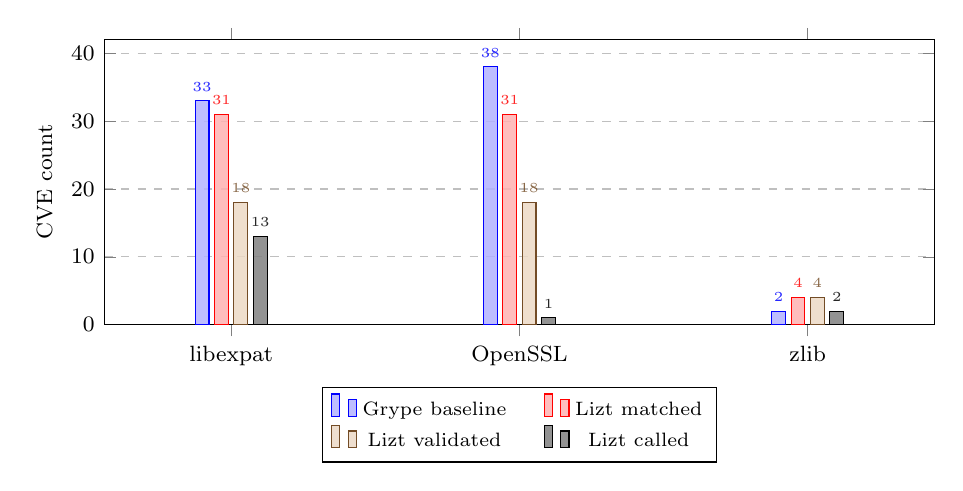
\begin{tikzpicture}
    \begin{axis}[
      ybar,
      bar width=5pt,
      width=\columnwidth,
      height=5.2cm,
      enlarge x limits=0.22,
      ylabel={CVE count},
      ylabel style={font=\footnotesize},
      symbolic x coords={libexpat, OpenSSL, zlib},
      xtick=data,
      xticklabel style={font=\footnotesize},
      yticklabel style={font=\footnotesize},
      ymin=0,
      ymax=42,
      legend style={
        at={(0.5,-0.22)},
        anchor=north,
        legend columns=2,
        font=\scriptsize,
        /tikz/every even column/.append style={column sep=0.4cm},
      },
      ymajorgrids=true,
      grid style=dashed,
      every axis plot/.append style={fill opacity=0.85},
      nodes near coords,
      nodes near coords style={font=\tiny, /pgf/number format/.cd,fixed,precision=0},
    ]
    \addplot coordinates {(libexpat,33) (OpenSSL,38) (zlib,2)};
    \addplot coordinates {(libexpat,31) (OpenSSL,31) (zlib,4)};
    \addplot coordinates {(libexpat,18) (OpenSSL,18) (zlib,4)};
    \addplot coordinates {(libexpat,13) (OpenSSL,1)  (zlib,2)};
    \legend{Grype baseline, Lizt matched, Lizt validated, Lizt called}
    \end{axis}
  \end{tikzpicture}
  \caption{CVE reduction funnel per library. \emph{Grype baseline} is the CPE-only count; \emph{matched} are CVEs whose version range passes Lizt's local verifier; \emph{validated} retain at least one symbol confirmed in the binary's symbol table;
    \emph{called} had at least one uprobe fire during the fixture
    workload.}
  \label{fig:cve-funnel}
\end{figure}

The baseline-to-matched step (73~$\to$~66) reflects Lizt's local version-range verifier catching CPE-range mismatches that the NVD endpoint returned but that do not actually apply to the installed version. The matched-to-validated step (66~$\to$~40) is the largest absolute reduction and corresponds to the symbol-validation pass described in \S\ref{sec:sysdesign}: of the 66 CVEs whose version matched, only 40 had at least one scraped symbol that was also present in the target binary's symbol table. The remaining 26 are not false positives of the CPE match itself---the version genuinely falls in the vulnerable range---but they are findings for which Lizt has no actionable runtime confirmation path, either because the symbol was never extractable (description too terse, no linked patch diff) or because the symbol exists only as a static or inlined function inaccessible to named uprobes. The validated-to-called step (40~$\to$~16) is the runtime-observation signal: 16 of the 40 instrumented CVEs had at least one probe fire during the fixture workload, while the remaining 24 were attached but never triggered.

End-to-end, Lizt reclassifies 78\% of Grype's baseline findings as either unreachable (symbol absent or never called) or not runtime-confirmed. Of the original 73 CVEs, 21.9\% remain as runtime-confirmed findings after the full pipeline; the remainder are retained in the database with their weaker \texttt{symbol\_present}/\texttt{symbol\_called} flags so that an operator can audit the distinction between ``present but not observed'' and ``absent entirely'' during triage.

\subsection{Per-Library Breakdown}

Figure~\ref{fig:cve-funnel} disaggregates the funnel per library. The three libraries exhibit markedly different behavior at the validated-to-called boundary:

\paragraph{libexpat (33~$\to$~31~$\to$~18~$\to$~13)}
The XML parser was the most active fixture: the evaluation workload (parsing a malformed XML document through the fixture binary) exercised attribute processing, content handling, and namespace-separator paths, causing 13 of 18 instrumented CVEs to fire at least one probe. This is the expected outcome for a library whose core API surface is densely packed with vulnerable entry points: any realistic parser invocation crosses multiple of them.

\paragraph{zlib (2~$\to$~4~$\to$~4~$\to$~2)}
The \texttt{matched} count exceeds the baseline because Lizt's alternative-CPE generator produces additional candidate entries (e.g., stripping the \texttt{lib} prefix) that resolve against NVD entries Grype's canonical-CPE match did not retrieve---a rare case where a reachability-oriented design also improves \emph{coverage}. Of the 4 validated CVEs, 2 fired during the workload (an \texttt{inflate} call on a crafted gzip stream), including CVE-2022-37434 whose patch commit (\texttt{eff308af}, a three-line diff) is the paper's gold-standard end-to-end exemplar.

\paragraph{OpenSSL (38~$\to$~31~$\to$~18~$\to$~1)}
OpenSSL produced the steepest drop from baseline to called: 38 CPE-matched CVEs, 18 with validated symbols, and 0 fired during the initial benign workload. This is not a failure of instrumentation; it is the expected behavior for a cryptographic library whose vulnerable paths are triggered by specific, often malformed, protocol inputs rather than ordinary TLS handshakes. The conditional reachability experiment in \S\ref{sec:conditional} isolates exactly this case.

\subsection{Fixture Correctness (RQ2)}

Table~\ref{tab:fixtures-expanded-results} reports end-to-end behavior on the five-CVE fixture suite introduced in \S\ref{sec:fixtures}.
\begin{table*}[t]
  \centering
  \caption{Fixture-level results. ``Symbols extracted'' is the
    count produced by the scraper for the named CVE; ``In
    \texttt{.dynsym}'' and ``In \texttt{.symtab}'' report presence
    in the binary's dynamic and full symbol tables; ``Uprobe
    fires'' indicates whether the named symbol was observed during
    the fixture workload.}
  \label{tab:fixtures-expanded-results}
  \begin{tabular}{llllccccl}
    \toprule
    \textbf{CVE}
      & \textbf{Software}
      & \textbf{Version}
      & \textbf{Target symbol}
      & \textbf{\shortstack{Symbols\\extracted}}
      & \textbf{\shortstack{In\\\texttt{.dynsym}}}
      & \textbf{\shortstack{In\\\texttt{.symtab}}}
      & \textbf{\shortstack{Uprobe\\fires}}
      & \textbf{Outcome} \\
    \midrule
    CVE-2022-37434 & zlib     & 1.2.11
      & \texttt{inflate}          & 2 & Yes & Yes & Yes & Fully confirmed \\
    CVE-2022-25315 & libexpat & 2.2.9
      & \texttt{storeRawNames}    & 1 & No  & Yes & Yes & Fully confirmed \\
    CVE-2022-40674 & libexpat & 2.2.9
      & \texttt{doContent}        & 1 & No  & Yes & Yes & Fully confirmed \\
    CVE-2022-25236 & libexpat & 2.2.9
      & \texttt{storeAtts}        & 1 & No  & Yes & Yes & Fully confirmed \\
    CVE-2022-0778  & OpenSSL  & 1.1.1f
      & \texttt{BN\_mod\_sqrt}    & 1 & Yes & Yes & Yes & Fully confirmed \\
    \bottomrule
  \end{tabular}
\end{table*}
CVE-2022-37434 (zlib) is the cleanest case. The description text names \texttt{inflate} and \texttt{inflateGetHeader} explicitly, the upstream fix (\texttt{madler/zlib} commit \texttt{eff308af}) is a three-line diff that both scrapers converge on, and both symbols are dynamically exported. The fixture workload decompresses a crafted gzip stream through \texttt{inflate}, causing the uprobe to fire within milliseconds of the workload starting. This is the end-to-end pipeline operating as designed: description scrape, patch-diff corroboration, dynamic-symbol validation, and runtime observation all agree.

The three libexpat CVEs (CVE-2022-25315, -40674, -25236) exercise a less obvious attachment path. The target symbols---\texttt{storeRawNames}, \texttt{doContent}, \texttt{storeAtts}---are declared \texttt{static} in \texttt{xmlparse.c} and are therefore absent from the shared library's dynamic symbol table: \texttt{readelf~-s} reports all three with \texttt{LOCAL} binding, invisible to \texttt{nm~-D}. They remain present in the full symbol table (\texttt{.symtab}) because the fixture binary was compiled with \texttt{CFLAGS="-g"} and not stripped. Aya's \texttt{UProbe::attach} resolves symbol names against both tables and computes the file offset from whichever match succeeds, so the attachment proceeds via \texttt{.symtab} without Lizt having to specify an explicit offset. The fixture workload (parsing a malformed XML document) triggered observations on all three symbols, and all three CVEs surface on the dashboard with \texttt{symbol\_called} set, scored above their CPE-match-only peers by the $2\times$ runtime multiplier (\S\ref{sec:database}). This result has implications for deployment on stripped binaries, discussed in \S\ref{sec:static-inlined}.

\subsection{Reachability vs. Exploitability: CVE-2022-0778}
\label{sec:conditional}

CVE-2022-0778 is a denial-of-service vulnerability in OpenSSL's \texttt{BN\_mod\_sqrt} function, reachable during certificate parsing but only exploitable when the certificate encodes a specially crafted elliptic-curve parameter that triggers an infinite loop in the modular square-root algorithm. The symbol is dynamically exported and the scraper extracts it correctly; the interesting question is whether Lizt over-reports the symbol on benign traffic or correctly surfaces it as a reachability finding in both scenarios.

We ran the fixture twice against the same binary and monitor session, varying only the workload:

\begin{enumerate}[noitemsep]
  \item \textbf{Benign workload.} A standard TLS handshake against a well-formed server certificate. \texttt{BN\_mod\_sqrt} was called 4~times during certificate-chain validation, terminating normally each time.
  \item \textbf{Malformed workload.} The same handshake against a certificate encoding the CVE-2022-0778 proof-of-concept parameter. \texttt{BN\_mod\_sqrt} was entered once and did not return within the observation window; the uprobe fired for entry but no corresponding return event was recorded.
\end{enumerate}

Both runs produce a \texttt{symbol\_called~=~true} finding for CVE-2022-0778, differing only in the return-event pattern. This is intentional. Lizt reports reachability, not exploitability; a return-pattern-based exploit oracle is out of scope (see Threat Model, \S\ref{sec:threat-model}). What the experiment does demonstrate is that the system correctly handles symbols reached on \emph{both} benign and malicious inputs without the former drowning out the latter: the vulnerability is surfaced in both cases, and the ranking function's $2\times$ \texttt{called} multiplier (\S\ref{sec:database}) pushes it above CPE-matched-only findings in either scenario. A concrete implication is that an operator running a long-lived service terminating TLS is told that CVE-2022-0778 is reachable on their system regardless of whether an attacker has yet sent the trigger, which is the correct triage posture for a denial-of-service primitive reached on every handshake.

\subsection{Overhead}

Uprobe instrumentation has a per-event cost but only a small steady-state footprint when probes are not firing. On the libexpat fixture with 18 attached uprobes and a parser workload saturating the CPU, the \texttt{lizt} process held steady at well under one percent of a core of background CPU when idle. During the active parser workload, overhead is dominated by the PostgreSQL upsert path rather than the kernel-side probe cost; this is by design, since the observation-upsert scheme (\S\ref{sec:database}) trades per-event write amplification for a bounded row count per \texttt{(cve\_symbol\_id, pid)} pair. A broader characterization of overhead under production workloads is identified as future work (\S\ref{sec:future-work}).


% ============================================================
\section{Discussion}
% ============================================================

\subsection{What the Reduction Means}

The headline 78\% reduction from the Grype baseline to runtime-confirmed findings should not be read as ``78\% of Grype's findings were wrong.'' It is more precisely the gap between two different questions: ``is a vulnerable version installed?'' (what Grype answers) and ``has vulnerable code executed on this system during the observation window?'' (what Lizt answers). The difference between those questions is the space in which operators currently spend their triage time, and the empirical result is that the space is large---of 73 CPE-matched findings on the fixture suite, only 16 carried runtime evidence of reachability during a realistic workload.

The converse framing matters equally. A finding that is present in the baseline but absent from the \texttt{called} column is not dismissed: it is retained in the database with weaker reachability flags so that a later scan---or a different workload---can promote it. Lizt's reduction is informational, not destructive.

\subsection{Stripped Binaries and Inlined Symbols}
\label{sec:static-inlined}

Lizt's reachability pipeline depends on the target binary retaining at least one symbol table containing the vulnerable function's address. The evaluation fixtures satisfy this in two distinct ways: \texttt{inflate} and \texttt{BN\_mod\_sqrt} are present in \texttt{.dynsym} as dynamically exported functions, while \texttt{storeRawNames}, \texttt{doContent}, and \texttt{storeAtts} are \texttt{static} in C source and appear only in \texttt{.symtab}. Both cases are handled by Aya's name-resolution path without Lizt specifying an explicit offset (\S\ref{sec:eval}).

Two cases fall outside this coverage. The first is fully stripped binaries, where both \texttt{.dynsym} and \texttt{.symtab} have been removed; on such targets, uprobe attachment requires DWARF debug information from a separate \texttt{.debug} file or detached symbol package to resolve function names to file offsets. The second is aggressively inlined functions, which have no standalone address at all: a call site is expanded into the caller's instruction stream, leaving no single instruction boundary for a probe to attach to. The only recourse in the inlined case is source-level instrumentation via call-graph analysis of the nearest non-inlined caller, which trades probe-attachment simplicity for call-graph complexity. Both cases are documented in Future Work (\S\ref{sec:future-work}).

\subsection{Threat Model and Claims}
\label{sec:threat-model}

Lizt claims that, within a given observation window, a listed symbol was entered at least once during a process' execution. It does not claim that the entry was triggered by an attacker, that the surrounding preconditions for exploitation were satisfied, or that the absence of an observation implies safety. The CVE-2022-0778 experiment (\S\ref{sec:conditional}) makes this explicit: \texttt{BN\_mod\_sqrt} is called during routine certificate validation, so a \texttt{symbol\_called} finding does not by itself indicate exploitation.

The corollary is that Lizt is a triage and prioritization tool, not a proof of exploitability or a replacement for manual security review. Its value in the workflow is upstream of those activities: it narrows the set of findings on which an analyst must exercise judgment, and it surfaces the distinction between ``vulnerable code is linked in but dormant'' and ``vulnerable code is actively executed'' so that the latter can be prioritized for deeper review.

\subsection{Observation Window}

All results in \S\ref{sec:eval} are conditioned on a fixture-scoped observation window in which the vulnerability's exercise path was deliberately triggered. A production deployment faces a different problem: workloads vary over time, and a symbol that is never called on Monday may fire on Tuesday. Lizt's current design accommodates this through the \texttt{last\_seen} column in the \texttt{symbol\_activity} materialized view, which records the most recent observation timestamp per symbol. Operators can therefore distinguish ``never observed'' from ``observed last week but quiet since,'' which has different triage implications. A longer-running empirical study of observation-window dynamics on production workloads is the natural next step and is identified explicitly in \S\ref{sec:future-work}.

\subsection{Comparison with Static Reachability}

A fair comparison is with static call-graph reachability analysis, as implemented commercially by Snyk~\cite{snyk} and similar tools. Static reachability answers ``could the vulnerable function be called from application code?'' via source-level call graph analysis; Lizt answers ``was it called?'' via runtime observation. The two are complementary rather than competitive: static analysis over-approximates (every reachable path is reported regardless of whether it executes in practice) while runtime observation under-approximates (only paths exercised during the observation window are reported). A hybrid deployment---static reachability as an upper bound, Lizt as a lower bound---produces a tighter actionable set than either alone, and bridging the two through shared CVE-to-symbol metadata is an appealing direction for future work.

\subsection{Threats to Validity}

\emph{Construct validity.} The fixture library is small (three source-compiled libraries, five headline CVEs) and deliberately chosen for symbol-extraction tractability. All fixture binaries retain both \texttt{.dynsym} and \texttt{.symtab}; stripped production binaries would require DWARF-guided resolution (\S\ref{sec:static-inlined}) not exercised here, and the headline reduction percentages are not directly generalizable to such workloads.

\emph{Internal validity.} The Grype baseline is measured with SBOM-mode invocation to force NVD CPE matching. Distribution-advisory resolution (the default path for system-package-installed libraries) would produce a different baseline---likely smaller, because distribution vendors backport fixes without bumping version strings~\cite{redhat_backporting}. The SBOM-mode configuration was chosen to isolate the version-range-matching behavior rather than the distribution advisory feed quality, but it does mean that results are not directly comparable to a default \texttt{grype dir:/} scan on a stock Ubuntu system.

\emph{External validity.} All fixtures run on a single Ubuntu~24.04 instance on AWS. Kernel version (6.8), glibc, and the specific compile flags on the target libraries all influence both \texttt{.dynsym} contents and probe attachment behavior. A full portability study across distributions and kernel versions is out of scope for this evaluation.


\subsection{Future Work}
\label{sec:future-work}

Several extensions are planned.

\emph{DWARF-guided uprobes for stripped binaries.} Aya's existing name-resolution path covers binaries retaining either \texttt{.dynsym} or \texttt{.symtab}. Stripped production binaries, where both tables have been removed, currently fall outside Lizt's coverage. A DWARF-based resolver reading debug info from separate \texttt{.debug} files or detached symbol packages would extend Lizt's reach to this case without changing the uprobe attachment mechanism.

\emph{Unmanaged binaries.} Source-compiled or side-loaded binaries are already detected by the \texttt{InstalledBinarySource} ELF scan, but operators sometimes want to declare them explicitly rather than rely on filesystem discovery. A \texttt{ManualSource} reading from \texttt{/etc/lizt/manual-installs.toml} would cover this case and would also allow pinning CPE assignments for binaries whose provenance is unambiguous.

\emph{OSV enrichment.} The OSV database~\cite{osv} is already queried during symbol extraction. Lifting OSV into a full enrichment layer on top of NVD (advisory-level detail, commit-level fix metadata, ecosystem-specific context) would improve both scraper coverage and the quality of the per-finding metadata presented in the dashboard.

\emph{Broader empirical benchmarking.} The headline evaluation uses three source-compiled libraries; a large-scale study across production container images and long-lived services would produce reduction-rate statistics grounded in real-world workloads rather than fixture workloads. This is the natural avenue for quantitative validation of Lizt's claimed benefit at scale.

\emph{Return-aware exploit oracles.} A return-tracing variant of the uprobe could record whether a vulnerable function ever fails to return within a bounded time---a primitive that would have correctly flagged the infinite-loop behavior in the malformed CVE-2022-0778 run. This is an exploitability signal, not merely a reachability signal, and expanding Lizt in this direction crosses the triage-to-detection boundary deliberately drawn in \S\ref{sec:threat-model}.


% ============================================================
\section{Conclusion}
% ============================================================

Traditional software composition analysis tools report vulnerabilities based on CPE-level version matching, which cannot distinguish between the presence of a vulnerable package and the reachability of its vulnerable code at runtime. On our fixture suite, this gap is substantial: 57 of 73 CPE-matched CVEs (78\%) carry no runtime evidence of reachability during realistic workloads. Lizt addresses this gap by layering eBPF uprobe monitoring on top of CPE matching, confirming whether vulnerable symbols are actually executed before promoting them to actionable findings. The evaluation demonstrates that the system correctly recognizes reachable paths (CVE-2022-37434 in zlib), flags static-symbol cases as instrumentation gaps rather than silently dropping them (the libexpat fixtures), and surfaces conditional-reachability vulnerabilities identically on both benign and malicious workloads (CVE-2022-0778 in OpenSSL)---leaving the exploitability determination to the operator while ensuring the finding is never lost.

Lizt is released as an open-source Rust toolchain: a unified Cargo workspace that includes the scanner, the nightly-Rust eBPF monitor, and a web-based findings dashboard that runs under a single systemd service. The evaluation numbers reported here are reproducible via the \texttt{lizt eval --fixture} subcommand against the fixture suite described in \S\ref{sec:fixtures}. Planned extensions---offset-based uprobes, manual-source declarations, OSV enrichment, and large-scale empirical benchmarking---target the limitations identified in \S\ref{sec:future-work} and, more broadly, the goal of pushing the runtime-confirmed fraction of the reduction funnel upward on libraries whose vulnerability surface is currently inaccessible to named-symbol instrumentation.
% ============================================================
\section*{Acknowledgments}
% ============================================================

Portions of Lizt's architecture, Rust implementation, evaluation methodology, and this paper were developed with the assistance of Claude~\cite{claude}, a large language model developed by Anthropic. Specifically, Claude was used for architectural design discussion, code generation and review, evaluation fixture planning, GUI design, and \LaTeX{} document preparation. All AI-generated output was reviewed, validated and adapted by the author.

% ============================================================
%  References
% ============================================================
\bibliographystyle{IEEEtran}
\bibliography{references}

\end{document}